\section{Microeconomics Midterm 2019 / 20}

{
\subsection*{Schmidt}

{
\subsubsection*{Exercise 1}

\begin{enumerate}[label=(\roman*)]
{\item 
First, find incomes:

$$
w^{0}=42 \quad w^{1}=36 \quad w^{2}=50
$$

Look for violations of WARP:

\begin{table}[!htp]
    \centering
    \begin{tabular}{|c|c|l|l|l|l|}
    \hline
    $t$ & $t^{\prime}$ & $p^{t} x^{t^{1}}$ & $\sum$ & $w^{t}$ & revealed preferences \\
    \hline \multirow{2}{*}{0} & 1 & $p^{0} x^{1}=48$ & $>$ & 42 & - \\
    \cline { 2 - 6 } & 2 & $p^{0} x^{2}=40$ & $<$ & 42 & $x^{0}>x^{2}$ \\
    \hline \multirow{2}{*}{1} & 0 & $p^{1} x^{0}=33$ & $<$ & 36 & $x^{1}>x^{0}$ \\
    \cline { 2 - 6 } & 2 & $p^{1} x^{2}=39$ & $>$ & 36 & - \\
    \hline \multirow{2}{*}{2} & 0 & $p^{2} x^{0}=52$ & $>$ & 50 & - \\
    \cline { 2 - 6 } & 1 & $p^{2} x^{1}=48$ & $<$ & 50 & $x^{2}>x^{1}$ \\
    \hline
    \end{tabular}
\end{table}

From the table we see that we never have $p^{t} x^{t^{\prime}} \leq w^{t}$ and $p^{t^{\prime}} x^{t} \leq w^{t^{\prime}}$. Therefore, WARP is satisfied.
}
{\item 
From the last row we have $x^{0}>x^{2}$ and $x^{2}>x^{1}$

Transitivity implies $x^{0}>x^{\prime}$ but we found the opposite: $x^{\prime}>x^{0}$. Therefore, transitivity is violated.
}
\end{enumerate}
}
{
\subsubsection*{Exercise 2}

\begin{enumerate}[label=(\alph*)]
{\item 
Consumer 1: at optimum $e_{1}(\cdot)=w_{1}$ \& $u_{1}=v_{1}(\cdot)$

$$
\begin{aligned}
w_{1} & =v_{1}\left(p, w_{1}\right) \sqrt{p_{1} p_{2}} \\
\Leftrightarrow v_{1}\left(p, w_1\right) & =\frac{w_{1}}{\sqrt{p_{1} p_{2}}}
\end{aligned}
$$

Use Roy's identity:

$$
\begin{aligned}
x_{1}^1(p, w) & =-\frac{\frac{\partial v_{1}\left(p_{1} w\right)}{\partial p_{1}}}{\frac{\partial v_{1}\left(p_{1} w\right)}{\partial w_{1}}}=-\frac{-\frac{1}{2} \frac{w_{1}}{\sqrt{p_{2}} p_{1}^{-3 / 2}}}{\frac{1}{\sqrt{p_{1} p_{2}}}} \\
& =\frac{w_{1}}{2 p_{1}}
\end{aligned}
$$

By symmetry: $x_{2}^1\left(p_{1} w\right)=\frac{w_{1}}{2 p_{2}}$

Consumer 2: Transform utility function.

$$
u_{2}\left(x_{1}, x_{2}\right)=x_{1}^{\frac{3}{3+a}} x_{2}^{\frac{a}{3+a}}
$$

This is standard Cobb-Dauglas:

$$
x_{1}^{2}(p, w)=\frac{3}{3+a} \frac{w_{2}}{p_{1}} ; x_{2}^1 (p, w)=\frac{a}{3+a} \frac{w_{2}}{p_{2}}
$$
}
{\item 
Good 1: $\quad x_{1}^{1}+x_{1}^{2}=\frac{1}{p_{1}}\left[\frac{1}{2} w_{1}+\frac{3}{3+a} w_{2}\right]$

$$
\longrightarrow \frac{1}{2}=\frac{3}{3+a} \Longleftrightarrow a=3
$$

Good 2: $x_{2}^{1}+x_{2}^{2}=\frac{1}{p_{2}}\left[\frac{1}{2} w_{1}+\frac{a}{3+a} w_{2}\right]$

$$
\longrightarrow \frac{1}{2}=\frac{a}{3+a} \Longleftrightarrow a=3
$$

Thus $a=3$ solves the problem for both goods.
}
\end{enumerate}
}
{
\subsubsection*{Exercise 3}

\begin{enumerate}[label=(\alph*)]
{\item 
Firm solves:

\begin{align*}
    \min _{x} c(w, y) = \min_x w x \\
    \text { s.t. } f(x)=y
\end{align*}

FOC:

\begin{align*}
    w_{l}=\lambda \frac{\partial f(x)}{\partial x_{l}} \quad \forall l
\end{align*}

Use Euler:

\begin{align*}
    c(w, y)=\lambda \sum_{l} \frac{\partial f(x)}{\partial x_{l}} x_{l}=\lambda f(x)=\lambda y
\end{align*}

If $y=1: c(w, 1)=\lambda$

If $y \neq 1: c(w, y)=\lambda y=c(w, 1) y=c(w) y$
}
{\item 
We have:

$$
\begin{aligned}
& c(w, y)=w x \\
& \frac{\partial(w, y)}{\partial w_{l}}=\frac{\partial w x}{\partial w_{l}}=x_{l}
\end{aligned}
$$

And from (a):

$$
\frac{\partial c(w, y)}{\partial w_{l}}=\frac{\partial c(w, 1)}{\partial w_{l}} y
$$

Together:

$$
x_{l}=\frac{\partial c\left(w, 1\right)}{\partial w_{l}} y
$$
}
{\item 
Profits are:

$$
\pi=p f(x)-w x=p f(x)-\sum_{l} w_{l} x_{l}
$$

Plug in the $w_l$ from exercise

$$
\begin{aligned}
\pi & =p f(x)-\sum_{l} p \frac{\partial f(x)}{\partial x_{l}} x_{l} \\
& =p\left[f(x)-\sum_{l} \frac{\partial f(x)}{\partial x_{l}} x_{l}\right]=p[f(x)-f(x)]
\end{aligned}
$$

The last equality follows from CRS \& Euler's formula. Clearly, $\pi=0$.
}
\end{enumerate}
}
{
\subsubsection*{Exercise 4}

\begin{enumerate}[label=(\roman*)]
{\item 
DM maximize expected utility:

$$
\begin{aligned}
\max _{\alpha, \beta} E U(\cdot) & =\max _{\alpha, s} \int u(w-\alpha-\beta+\alpha z+\beta) d F(z) \\
& =\max _{\alpha} \int u(w-\alpha+\alpha z) d F(z)
\end{aligned}
$$

Get first order derivative:

$$
\frac{\partial E U}{\partial \alpha}=\int u^{\prime}(w-\alpha+\alpha z)(z-1) d F(z)
$$

Suppose $\alpha=0$ :

$$
\begin{aligned}
& \int u^{\prime}(w)(z-1) d F(z)
= u^{\prime}(w)\left[\int z d F(z)-1\right]>0
\end{aligned}
$$

As the expected marginal utility is positive at $\alpha=0$, the DM will invert some $\alpha>0$.
}
{\item 
As we saw in (i), $\alpha=0$ is not optimal (for both agents). They increase $\alpha$, which lowers the marginal expected utility, until $\frac{\partial E U}{\partial \alpha}=0$.
Because $v(\cdot)$ is a concave transformation of $u(\cdot)$, we know that $v^{\prime}(\cdot)$ decreases faster then $u^{\prime}(\cdot)$.
Therefore, $\int v^{\prime}(\cdot)(z-1) d F(z)=0$ is reached at a lower value of $\alpha$ than for $\int u^{\prime}(\cdot)(z-1) d F(z)$. Thus:

$$
\alpha_{v}^{*}<\alpha_{u}^{*}
$$
}
\end{enumerate}
}
}

{
\subsection*{Gottardi}

{
\subsubsection*{Exercise 1}

\begin{enumerate}[label=(\roman*)]
{\item 
\underline{Consumer A:}

\begin{align*}
\max _{x_1^A, x_2} x_1^A x_2^A \text { s.t. } p x_1^A+x_2^A=p 8
\end{align*}

FOCs

\begin{align*}
    {\left[x_1^A\right]:} & x_2^A-\lambda p=0 \\
    {\left[x_2^A\right]:} & x_1^A-\lambda=0 \\
    \rightarrow& x_2^A=p x_1^A\tag{I}
\end{align*}

Combine (I) with BC:

\begin{align*}
    x_1^A=4 \quad ; \quad x_2^A=4 p
\end{align*}

\underline{Consumer B:}

\begin{align*}
    \max _{x_{1}^{B} x_{3}^{B}} x_{1}^{B}+2 x_{2}^{B} \text{ s.t. }p x_{1}^{B}+x_{2}^{B}=6
\end{align*}

By linearity:

$$
\begin{aligned}
& x_{1}^{B}=\left\{\begin{array}{lll}
\infty & \text { if } & p<1 / 2 \\
\mathbb{R}^{+} & \text {if } & p=1 / 2 \\
0 & \text { if } & p>1 / 2
\end{array}\right. \\
& x_{2}^{B}=\left\{\begin{array}{lll}
\infty & \text { if } & p>1 / 2 \\
\mathbb{R}^{+} & \text {if } & p=1 / 2 \\
0 & \text { if } & p<1 / 2
\end{array}\right.
\end{aligned}
$$

\underline{Markets:}

$p=1 / 2$ otherwise we would have excess demand for one of the goods.

$$
\begin{aligned}
    & \longrightarrow x_{2}^{A}=2 \\
    & \longrightarrow x_{1}^{B}=8-4=4 \\
    & \longrightarrow x_{2}^{B}=6-2=4 \\
\end{aligned}
$$

\underline{Competitive Equilibrium:}

$$
\begin{aligned}
    & \left(x_{1}^{A}, x_{2}^{A}\right)=(4,2) \\
    & \left(x_{1}^{B}, x_{2}^{B}\right)=(4,4) \\
    & p=\frac{1}{2}
\end{aligned}
$$
}
{\item 
$M RS^{A}=x_{2}^{A} / x_{1}^{A} \stackrel{!}{=} M R S^{B}=1 / 2 \longrightarrow x_{2}^{A}=\frac{1}{2} x_{1}^{A}$ in blue:

\begin{figure}[!htp]
    \centering
    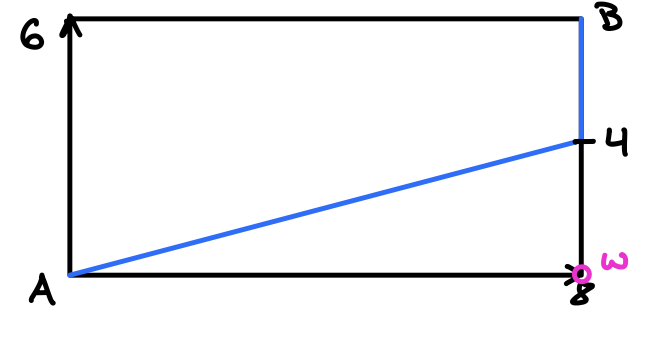
\includegraphics[width=.5\textwidth]{images/2019_20_1.png}
\end{figure}
}
\end{enumerate}
}
{
\subsubsection*{Exercise 2}

\begin{enumerate}
    \item LNS of preferences
    \item complete markets
    \item free disposal
\end{enumerate}

Suppose (1) is violated. Then we could construct the following situation (A violates LNS):

\begin{figure}[!htp]
    \centering
    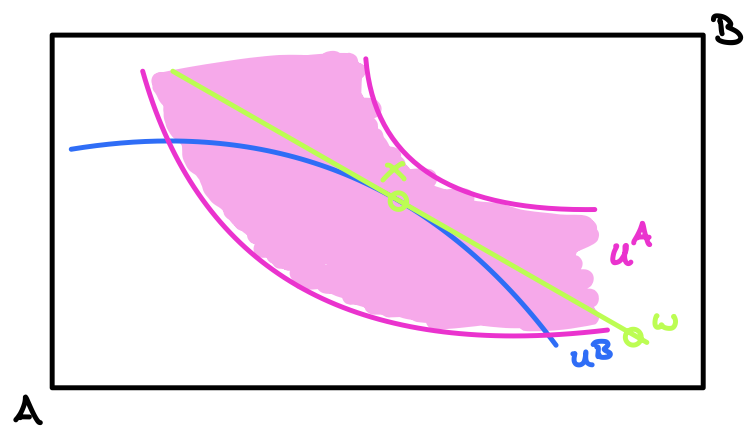
\includegraphics[width=.75\textwidth]{images/2019_20_2.png}
\end{figure}

Although at $x$ both agents are optimizing given the prices, we could make $B$ better off without hurting $A$ if we moved to the bottom left. Thus the CE at $x$ is not PE.
}
{
\subsubsection*{Exercise 3}

\begin{align*}
    \left(w_{1}, w_{2}\right)=(9,16)
\end{align*}

\begin{enumerate}[label=(\alph*)]
{\item 
$$
\begin{array}{ll}
t=0: & q_{1} \theta_{1}+q_{2} \theta_{2}=0 \\
t=1 \text { and } s=1: & x_{1}=w_{1}+\theta_{1}+3 \theta_{2}=9+\theta_{1}+3 \theta_{2} \\
t=1 \text { and } s=2: & x_{2}=w_{2}+3 \theta_{1}+\theta_{2}=16+3 \theta_{1}+\theta_{2}
\end{array}
$$
}
{\item 
Solve the maximization problem. I already substitute $x_{1}$ and $x_{2}$ from the BC s into the EU-function :

$$
\begin{gathered}
\max _{\theta_{1} \theta_{2}} \frac{1}{2}\left[\sqrt{9+\theta_{1}+3 \theta_{2}}+\sqrt{16+3 \theta_{1}+\theta_{2}}\right] \\
\text { st. } \quad q_{1} \theta_{1}+q_{2} \theta_{2}=0
\end{gathered}
$$

FOC:

$$
\begin{aligned}
& \frac{1}{2}\left[\frac{1 / 2}{\sqrt{9+\theta_{1}+3 \theta_{2}}}+\frac{1 / 2 \cdot 3}{\sqrt{16+3 \theta_{1}+\theta_{2}}}\right]-\lambda q_{1}=0 \\
& \frac{1}{2}\left[\frac{1 / 2 \cdot 3}{\sqrt{9+\theta_{1}+3 \theta_{2}}}+\frac{1 / 2}{\sqrt{16+3 \theta_{1}+\theta_{2}}}\right]-\lambda q_{2}=0
\end{aligned}
$$

Since there is only one consumer. must have no trade equilibrium: $\theta_{1}=\theta_{2}=0$. Plug into FOCs:

$$
\begin{aligned}
    \frac{1}{2}\left[\frac{1 / 2}{3}+\frac{1 / 2 \cdot 3}{4}\right]-\lambda q_{1}=0 &\Longleftrightarrow \lambda q_{1}=\frac{1}{4}\left[\frac{1}{3}+\frac{3}{4}\right]=\frac{13}{4 \cdot 12} \\
    \frac{1}{2}\left[\frac{1 / 2 \cdot 3}{3}+\frac{1 / 2}{4}\right]-\lambda q_{2}=0 &\Longleftrightarrow \lambda q_{2}=\frac{1}{4}\left[1+\frac{1}{4}\right]=\frac{5}{4 \cdot 4} \\
    \longrightarrow & \frac{q_{1}}{q_{2}}=\frac{13}{12} \cdot \frac{4}{5}=\frac{13}{15}
\end{aligned}
$$
}
{\item 
$\mathbb{E}\left(r_{1}\right)=\frac{1}{2}(1+3)=2=\mathbb{E}\left(r_{2}\right)=\frac{1}{2}(3+1)$

Thus:

$$
\frac{q_{1}}{q_{2}}<1 \Longleftrightarrow \frac{1}{q_{2}}<\frac{1}{q_{1}} \Leftrightarrow \frac{\mathbb{E}\left(r_{1}\right)}{q_{1}}>\frac{\mathbb{E}\left(r_{2}\right)}{q_{2}}
$$

The expected rate of return for asset 1 is larger than for asset 2.

Since the consumer is richer in state 2 and risk-averse, she would like to buy asset 2 as insurance. Because she is alone in the economy, this demand for asset 2 increases $q_{2}$ relative to $q_{1}$. This in turn leads to $\frac{1}{q_{1}}>\frac{1}{q_{2}}$ and $\frac{\mathbb{E}\left(r_{1}\right)}{q_{1}}>\frac{\mathbb{E}\left(r_{2}\right)}{q_{2}}$.
}
\end{enumerate}
}
}